\documentclass[tikz,border=2pt]{standalone}
\usepackage[T1]{fontenc}
\usepackage{tgheros}
\renewcommand{\familydefault}{\sfdefault}
\usetikzlibrary{fit,positioning}
\pgfdeclarelayer{ps}
\pgfdeclarelayer{ms}
\pgfdeclarelayer{cor}
\pgfsetlayers{ps,ms,cor,main}

\definecolor{psblue}{HTML}{6FA8DC}
\definecolor{msgreen}{HTML}{B6D7A8}
\definecolor{correlatedred}{HTML}{EA9999}
\definecolor{infopurple}{HTML}{B4A7D6}
\definecolor{xdsorange}{HTML}{F6B26B}
\definecolor{optionalorange}{HTML}{F9CB9C}

\begin{document}
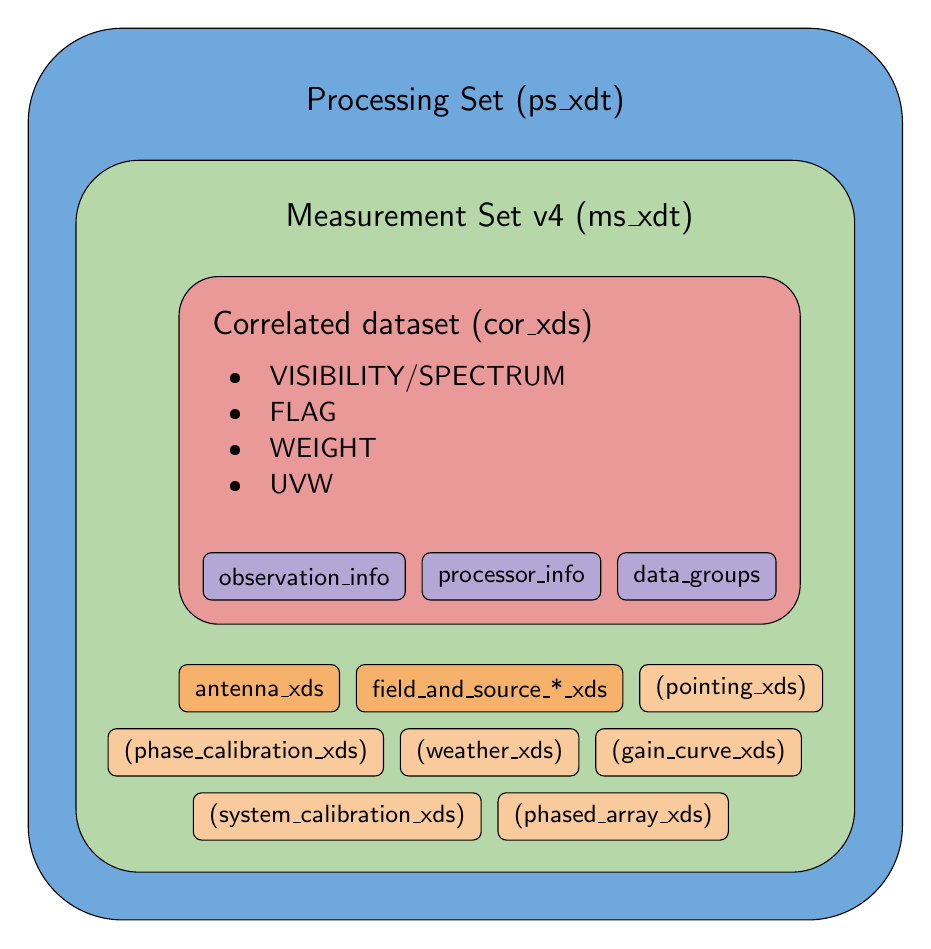
\begin{tikzpicture}[
    font=\small,
    item/.style={draw, rounded corners=3pt, minimum height=6mm, inner xsep=2mm},
    info/.style={item, fill=infopurple},
    xds/.style={item, fill=xdsorange},
    optional/.style={item, fill=optionalorange},
    container/.style={draw, fill=#1, inner sep=4mm},
    title/.style={font=\large},
    node distance=2mm,
  ]
  \node[title, anchor=north west] (cor title) at (0, 0)
    {Correlated dataset (cor\_xds)};
  \node[anchor=north west, align=left, font=\normalsize] (vars) at (0.2, -0.7)
    {\textbullet\quad VISIBILITY/SPECTRUM\\[1pt]
     \textbullet\quad FLAG\\[1pt]
     \textbullet\quad WEIGHT\\[1pt]
     \textbullet\quad UVW};
  \node[info, anchor=north west] (observation) at (0, -3.2) {observation\_info};
  \node[info, right=of observation] (processor) {processor\_info};
  \node[info, right=of processor] (data groups) {data\_groups};
  \begin{pgfonlayer}{cor}
    \node[container=correlatedred, rounded corners=5mm, inner sep=3mm,
      fit=(cor title) (vars) (observation) (processor) (data groups)] (cor) {};
  \end{pgfonlayer}

  \node[xds, below=5mm of cor] (field) {field\_and\_source\_*\_xds};
  \node[xds, left=of field] (antenna) {antenna\_xds};
  \node[optional, right=of field] (pointing) {(pointing\_xds)};
  \node[optional, below=of field] (weather) {(weather\_xds)};
  \node[optional, left=of weather] (phase cal) {(phase\_calibration\_xds)};
  \node[optional, right=of weather] (gain curve) {(gain\_curve\_xds)};
  \node[optional, below=of weather.south, anchor=north east, xshift=-1mm]
    (sys cal) {(system\_calibration\_xds)};
  \node[optional, below=of weather.south, anchor=north west, xshift=1mm]
    (phased array) {(phased\_array\_xds)};

  \node[title, above=4mm of cor] (ms title) {Measurement Set v4 (ms\_xdt)};
  \begin{pgfonlayer}{ms}
    \node[container=msgreen, rounded corners=8mm,
      fit=(ms title) (cor) (antenna) (pointing) (phase cal) (gain curve)
        (sys cal) (phased array)] (ms) {};
  \end{pgfonlayer}

  \node[title, above=4mm of ms] (ps title) {Processing Set (ps\_xdt)};
  \begin{pgfonlayer}{ps}
    \node[container=psblue, rounded corners=12mm, inner sep=6mm,
      fit=(ps title) (ms)] {};
  \end{pgfonlayer}
\end{tikzpicture}
\end{document}
